\documentclass[border=4pt]{standalone}
\usepackage{amsmath,amssymb,amsfonts}
\usepackage{xcolor,colortbl,array,booktabs,multirow}
\usepackage{tikz}
\usetikzlibrary{arrows, automata, backgrounds, calendar, chains, decorations,
    matrix, mindmap, patterns, petri, positioning, shadows, shapes.geometric,
    trees, shapes, decorations.pathreplacing, calc, tikzmark, arrows.meta}
\newcommand{\st}{\text{ s.t. }}
\newcommand{\x}{\mathbf{x}}
\renewcommand{\b}{\mathbf{b}}
\newcommand{\A}{\mathbf{A}}
\newcommand{\R}{\mathbb{R}}
\newcommand{\RR}{\mathbb{R}}
\newcommand{\Z}{\mathbb{Z}}
\newcommand{\ZZ}{\mathbb{Z}}
\begin{document}
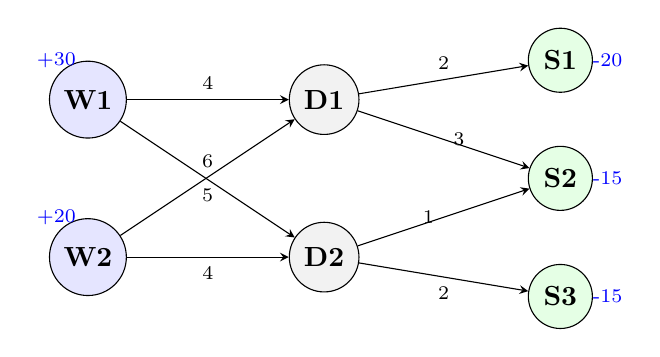
\begin{tikzpicture}[>=stealth, node distance=2cm]

% Warehouses
\node[draw, circle, fill=blue!10] (W1) at (0,2) {\textbf{W1}};
\node[draw, circle, fill=blue!10] (W2) at (0,0) {\textbf{W2}};

% Distribution Centers
\node[draw, circle, fill=gray!10] (D1) at (3,2) {\textbf{D1}};
\node[draw, circle, fill=gray!10] (D2) at (3,0) {\textbf{D2}};

% Stores
\node[draw, circle, fill=green!10] (S1) at (6,2.5) {\textbf{S1}};
\node[draw, circle, fill=green!10] (S2) at (6,1) {\textbf{S2}};
\node[draw, circle, fill=green!10] (S3) at (6,-0.5) {\textbf{S3}};

% Arcs with costs
\draw[->] (W1) -- (D1) node[midway, above] {\scriptsize 4};
\draw[->] (W1) -- (D2) node[midway, below] {\scriptsize 5};
\draw[->] (W2) -- (D1) node[midway, above] {\scriptsize 6};
\draw[->] (W2) -- (D2) node[midway, below] {\scriptsize 4};
\draw[->] (D1) -- (S1) node[midway, above] {\scriptsize 2};
\draw[->] (D1) -- (S2) node[midway, right] {\scriptsize 3};
\draw[->] (D2) -- (S2) node[midway, left] {\scriptsize 1};
\draw[->] (D2) -- (S3) node[midway, below] {\scriptsize 2};

% Supply/demand
\node[blue] at (-0.4,2.5) {\scriptsize +30};
\node[blue] at (-0.4,0.5) {\scriptsize +20};
\node[blue] at (6.6,2.5) {\scriptsize -20};
\node[blue] at (6.6,1) {\scriptsize -15};
\node[blue] at (6.6,-0.5) {\scriptsize -15};

\end{tikzpicture}
\end{document}
